\subsection{Module de curiosité}

Notre contrôleur mis en place, notre agent avait bien du mal à atteindre la moitié de l'environnement. Il est évident que l'apprentissage dans un environnement 3D était bien plus difficile. Pour nous convaincre de la difficulté d'un apprentissage sur un environnement labyrinthique, nous avons testé notre contrôle sur l'environnement de test Vizdoom (voir TODO section ?). Même constant, il est difficile pour l'agent d'explorer l'environnement et de dépasser la moitié de la carte.

Il y a deux explications naturelles à ce manque d'exploration:

\begin{enumerate}
\item L'agent ne reçoit qu'un état partiel de l'envrionnement et qui est déformé (passage 2D / 3D). 
\item Notre algorithme de contrôle ne contient aucun mécanisme poussant l'agent à explorer son environnment. Empiriquement, l'agent tourne en rond car l'A3C-LSTM-GAE favorise une uniformisation de la distribution de la politique. Dans notre cas, cela a pour effet d'avoir un agent qui va essayer toutes les actions (droite, gauche, haut, bas), et donc tourner en rond.
\end{enumerate}

Dans cette partie, nous allons expliquer comment fonctionne le module de curiosité qui a été mis en place. Nous commencerons par introduire succintement le dilemme exploration-exploitation, les différentes solutions dans le cadre de la théorie des Bandits à plusieurs armes et nous finirons pas discuter de la possibilité d'étendre les résultats au cadre de l'apprentissage par renforcement.

\subsubsection{La théorie des bandits à plusieurs bras}

Dans la théorie des bandits à plusieurs bras, un agent a un ensemble de K actions. A chaque action est associé une distribution $P_a$ de moyenne $\mu_a$. A chaque fois que l'agent choisit l'action a, il reçoit une récompense samplée depuis la distribution $P_a$ soit $r^t_a \sim P_a$. L'objectif de l'agent est de maximiser la somme des récompenses obtenues. 

$$
    \text{Maximiser: \: } \underset{t=1}{\overset{T}{\sum}}\:r^t_{a_i} \:\: \text{avec} \:\: r^t_{a_i}\sim P_a
$$

Il y a donc un paralèlle à faire entre le contexte de la théorie des bandits et celui de l'apprentissage par renforcement. Une dès grande différences est qu'en apprentissage par renforcement la distribution des récompenses est dépendante de la séquence d'action et possiblement dépendantes du temps. 

Nous nous intéressons dans cette partie à un contexte pour simple pour illustrer théoriquement le recours à un module de curiosité.

La notion de \textbf{regret} est centrale, et est défini comme la différence entre le choix optimal des actions et le choix de l'agent ($\text{Regret} = \underset{t=1}{\overset{T}{\sum}}\: \big( r_a_*^t - r^t_{a_i} \big) $).

L'idéal serait d'avoir un algorithme minimisant le regret obtenu par l'agent (trouver l'action qui mène à obtenir le maximum de récompenses). Au début, l'agent n'a évidemment pas idée des distributions $P_a$. Pour pouvoir estimer les dites distributions, il sera obliger d'effectituer des actions plus ou moins au hasard (d'\textbf{exploration} l'espace des actions). Toute la difficulté de la théorie des bandits et de savoir comment effectuer des actions de manière à explorer leur espace et savoir quand on a assez exploré pour exploiter la connaissance des estimés des distributions. 

La litérature concernant les bandits est riche néanmoins nous souhaitons justifier l'utilisation de mécanisme de curiosité via la théorie des bandits en montrant en quoi les stratégie naive son inéfficace. Ainsi, nous nous attarderons sur quatres stratégies populaires: les méthodes \textbf{Aléatoire}, \textbf{greedy}, \bm{\epsilon}\textbf{-greedy}, et\ \textbf{UCB}.

\begin{enumerate}
\item \textbf{La sélection d'actions aléatoire.}\\
C'est la stratégie la plus simple qui consiste à aléatoirement choisir une action. Cette stratégie est inefficace pour plusieurs raisons, la plus importante est qu'elle ne prend en compte les récompenses obtenues antérieurement.
Le regret espéré avec la méthode aléatoire est égale à: $T \big(\:\mu^* - \overset{\sim}{\mu}\: \big)$. Le regret croit de manière linéaire avec cette méthode, ce qui indique l'incapacité de cette méthode à trouver l'action optimale (ce qui est évident compte tenu de la méthode)
\item \textbf{La sélection d'actions selon la méthode greedy}\\
    La méthode greedy (pour avide) est une méthode de selection qui se contente de selectionner l'action qui à l'instant t, selon l'estimation de l'agent, donne la meilleur espérence de gain (de façon plus formelle $ a = \underset{a}{\text{argmax}} Q[a]$, avec Q le gain espéré estimé). Le problème est donc que l'agent va choisir continuellement un action dès lors qu'il n'aura plus d'égalité en espérence de gain selon les actions. Or, il est fort problème que l'estimation de l'agent soit mauvaise et donc qu'il se trompe d'action optimale. Avec cette méthode, le regret espéré est de: $T \big(\:\mu^* - \overset{\sim}{\mu_{a_i'}}\: \big)$, avec $i'$ l'action choisie en premier. Sans surprise, le reget crois de manière linéaire.
\item \textbf{La sélection d'actions selon la méthode} \bm{\epsilon} \textbf{-greedy} \\
    La\ méthode\ $\epsilon$-greedy est une variante de la méthode greedy dans laquelle l'action est choisie de façon greedy avec une probabilité de 1-$\epsilon$ et de façon aléatoire avec une probabilité $\epsilon$. Nous avons une borne inférieur de regré espéré qui est de $T \epsilon \big(\:\mu^* - \overset{\sim}{\mu}\: \big)$. Dans ce cas, le regret croit aussi de manière linéaire néanmoins nous voyant que si nous pouvons faire décroitre $\epsilon$ alors il serait théoriquement possible de faire croitre le regret seulement de façon logarithmique. C'est la méthode de sélection utilisé dans le \textbf{Deep-Q-Learning} et ses variantes. 

\item \textbf{La selection d'actions selon la stratégie UCB} \\
    \gls{UCB} pour \emph{Upper-Confidence-Bound} repose sur le principe d'optimisme face à l'incertitude. Ce principe stipule que plus nous sommes incertain de notre estimation sur le gain espéré plus il faut explorer cette action. On peut montrer théoriquement que dans le contexte des bandits simples, cela correspond à choisir de façon greedy plus un facteur de motivation à l'exploration. Soit formellement: 
    $$ \text{action} = \underset{a}{\text{argmax}}\bigg[Q[a] + \text{Curiosité}\bigg]  $$
    avec $\text{Curiosité} = \sqrt\frac{2\log t}{N(a)}$. On peut montrer que le regret croit de façon logarithmique ce qui est mieux que les stratégies précédantes.
\end{enumerate}


On pourrait donc imaginer utilisé une variante de l'\gls{UCB} dans le cadre de notre projet de contrôle. Néanmois, les formules données ci dessus ne sont valables que dans le cadre restreint au bandits. 
Sans pour autant utiliser \gls{UCB}, on pourra partir de cette idée de nécessité une motivation auxiliaire poussant l'agent à explorer l'environnement. Dans la partie suivante, nous allons tacher de définir plus précisement ce que veut dire d'explorer un environnement et nous allons proposer un module de curiosité pour arriver au contrôle de notre agent.

\subsubsection{Exploration et Motivation auxiliaire}

Le besoin d'exploration vient du simple fait que pour estimer la fonction d'état (ou d'état action), il faut avoir déjà recontré l'état visé. Or, dans le cas d'un environnement où l'agent n'a accès qu'a une vue partielle de l'environnement il est difficile d'estimer ces fonctions pour chaque état. Il apparait donc nécessaire de pousser l'agent à explorer en partie l'envrionnement pour déterminer au mieux une politique. Commne nous l'avons vu, dans la partie précédente, l'utilisation d'une récompense auxiliaire poussant à explorer l'environnement à du sens. Néanmoins, dans le contexte de l'apprentissage par renforcement les stratégies du style UCB (ou Bayesienne avec le sampling de Thomson) sont difficilement réalisable.

Pourtant, ce n'est pas la seule difficulté, l'état que reçoit notre agent est une représentation partielle de l'environnement. En effet, l'agent ne voit qu'un représentation 2D d'un environnement 3D. La question est donc de savoir comment explorer à partir d'une représentation compréssée de l'état. Cette problématique est au centre de la récherche en apprentissage par renforcement. Il y a plusieurs piste envisagées.

\begin{enumerate}
    \item Objectifs secondaires aidant l'agent dans ça prise de décision. Par exemple, nous pourrions optimiser notre réseau de neurones pour qu'il maximise la réduction de profondeur ($\text{depth}_{s1} > \text{depth}_{s2}$). Le problème de cette approche est qu'elle est dépendante de l'environnement.Or l'utilisation de l'apprentissage par renforcement est intéressante car elle permet d'être applicable à un grand nombre d'environnement sans grand changement.
    \item Formaliser le concepte d'exploration de façon générique. Nous chercherons une manière d'explorer un environnement à partir d'une représentation latente (compréssée) de celui ci. Il n'y a pas de consensus sur ce sujet actuellement.

    \item Utiliser des objectifs secondaires génériques. Par exemple, si nous pouvions formaliser de manière même simpliste la notion de curiosité, on peut faire l'hypothèse aurait pour effet une amélioration des performences l'algorithme car il en découlerait une exploration.
\end{enumerate}

\begin{figure}[h!]
\begin{center}
    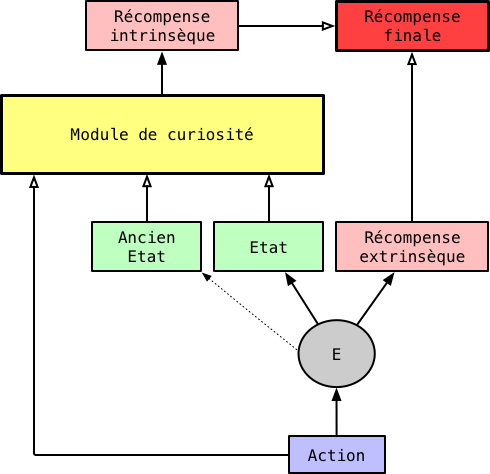
\includegraphics[scale=.5]{./assets/CURIOSITY/curiosity.png}
    \caption{Structure d'un module de curiosité}
\end{center}
\end{figure}

\subsection{Motivations auxiliaires et motivations}

Les motivations auxiliaires ont pu but d'aider l'agent à explorer son environnement. En effet, plus l'état est dimensionnelle élevée plus cela nécessite des approches particulières pour garantir que l'agent va être pousser à explorer celui-ci. Sans module auxiliaire, il est possible que l'agent reste dans un périmêtre restreint ce qui n'est pas souhaitable.

\subsubsection{Motivations auxiliaires spécifiques au environnements 3D}

Dans un premiers temps, nous allons explorer un module de curiosité simple que nous permettra d'introduire plus tard le module de curiosité qui a été integré dans le contrôle. Ce module par d'un constat simple,en poussant l'agent à changer en permanance le flux d'entrée qu'il perçoit, l'agent devra explorer l'environnement. En effet, bien souvent un manque d'exploration implique que les états que voient l'agent resteront similaire. Si l'agent recherche des états qui sont différents les uns des autres alors on peu faire l'hypothèse que l'agent sera pousser à explorer en profondeur l'environnements pour continuer de changer son flux d'entrée.

Formellement sela consiste à prendre la différence entre deux états sucessifs et considérer leurs normes comme un signal pouvant aider l'agent.

\begin{equation}
\text{récompense intrinsèque} = \lambda \: \norm{s_1 - s_2}^2 
\label{eqn:intrinsicmotivation}
\end{equation}

L'équation ~\autoref{eqn:intrinsicmotivation} est trop simple pour être utiliser. En effet, prenons le cas d'un agent qui tourne en rond, alors selon l'équation \ref{eqn:intrinsicmotivation} l'agent serait encouragé à tourner. Ce comportememt exclu donc l'utilisation de ce type d'approche naive. Nous allons décrire une méthodequi se base sur l'intuition que nous avons developpé en utilisant une approche hiérarchique. L'idée est que l'agent dévelope un mécanisme d'attention lui permettant de savoir qu'elle sous-partie de l'état est intéressante et avec laquelle on peut employer la stratégie simpliste.
Formellement cela revient à apprendre la séquence des k tel quel:

\begin{equation} 
    \text{récompense intrinsèque} = \tau\: \frac{\norm{h_k \odot \big[ s_t - s_{t-1} \big]}^2}{\norm{s_t - s_{t-1}  }^2}  
\end{equation}

L'équation ~\eqref{hierarchicalcuriosity} montre comment utilisé seulement une sous partie de l'entrée pour calculer la récompense intrinsèque. Cette formule est utilisé dans le papier \emph{Feature Control as Intrinsic Motivation for Hierarchical Reinforcement Learning}\cite{hierarchicalcuriosity}
Nous ne détaillerons pas la méthode pour déterminer la séquence de k car elle est extrêmment similaire à la façon de determiner la séquence d'action à effectuer. Nous avons aussi créer une méthode qui généralise la précédente qui au lieu de choisir un k, pondère par un facteur choisi par l'agent l'ensemble des sous ensembles de l'état pour calculer la récompense intrinsèque.

Nous avions peur de déstabiliser le réseau avec ce genre de recompense, le choix des hyperparamètres ($\lambda$, $\tau$) nécessite du soin et de nombreux essais.

Les tests préliminaires ont montrés que cela ne destabilisé pas l'apprentissage, néanmoins cela mériterais plus de test pour être convaincu de cela.

\begin{figure}[h!]
    \begin{center}
        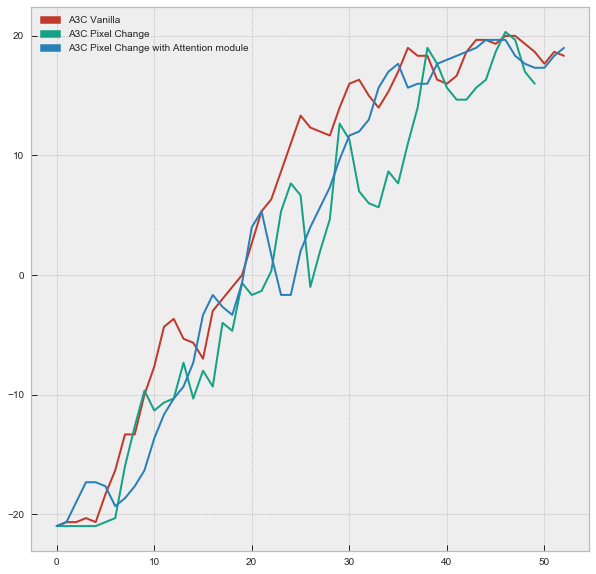
\includegraphics[scale=.35]{./assets/CURIOSITY/A3C_auxiliaire.png}
        \caption{Résultats des motivations auxiliaires sur Pong (Gym-OpenAI)}
    \end{center}
\end{figure}

Comme vous pouvez le voir le module a été testé avec comme contrôleur l'A3C. Les résultats indiquent que la recherche de la séquence de k pour un cas simple (Pong) n'augmente pas significativement l'entrainement. Il est reste maintenant a testé ce module avec SE-STAR. Les premiers résultats du contrôleur ne sont pas disponible avec ce module, il est noté que ce type de module n'a jamais été utilisé dans un cas aussi complexe qu'un environnement 3D crée par SE-STAR mais a été utilisé pour permettre à un agent d'explorer un environnement 2D qui nécessite une forte exploration et qui ne donne pas ou peu de signal intéressante pour l'apprentissage d'une politique optimale.

La solution présenté a été envisagé mais n'a pas été retenu dans le cadre du contrôle de l'agent. Nous avons utlisé un module de curiosité qui est plus générique.

\subsection{Module de curiosité générique intégré au contrôle}

Nous allons maintenant décrire la solution qui a été retenue dans le contrôle de SE-STAR. La solution proposée par des principes motivationnelles expliquées précédemment. La seule différence vient du faite que nous ne faisons plus un différence sur l'espace des pixels mais sur l'espace latent (construit par le réseau de neurone). L'avantage de cette méthode est de réussir à compresser l'état pour en extraire uniquement ce qui est indispensable. De plus, le module de curiosité utilise une méthode de compression supplémentaire qui a pour but de supprimer les parties qui ne sont pas influencé par l'action. Ce module est très fortement inspiré du papier \emph{Curiosity-driven Exploration in Deep Reinforcement Learning via Bayesian Neural Networks}\cite{curiositydriven}


Le module de curiosité est composé de plusieurs sous-modules:

\begin{itemize}
    \item \textbf{sous-module inverse}\\
        Le sous module inverse a pour but de trouver une compression permettant de réduire la dimensionnalité de l'état tout en étant capable de retrouver l'action qu'a effectué l'agent. Cela a pour but de travailler avec en entrée un nouvelle état qui est le plus pertinant possible. Imaginons le cas où l'agent se trouve devant un arbre, celui-ci aura les feuilles bougeants en permanence. Avec la stratégie de curiosité descrite précédemment il est alors aiséde voir que l'agent sera encouragé à ne pas bouger. Or, avec ce nouveau module de curiosité, comme l'agent ne peut agir sur les feuilles, ce sous module supprimer les feuilles et ainsi le module de curiosité aura un effet bien plus stable et ne sera pas sujet à des scénarios défavorables.
    \item \textbf{sous-module avant}\\
        Le sous module avant à pour but de déterminer la récompense intrinsèque qui sera donné à l'agent.
        En utilisant les compressions des états à l'instant t et t+1 que l'on nommera $\phi(s_t)$ et $\phi(s_{t+1}$), on peut appliquer la même stratégie que décrite dans le chapitre précédent. La récompense intrinsèques est donnée par la formule suivante:

\begin{equation}\label{eqn:hierarchicalcuriosity}
    \text{récompense intrinsèque} = \tau\: \norm{ \phi(s_t) - \phi(s_{t+1}) }^2 
\end{equation}

\end{itemize}

L'association permet d'utiliser notre stratégie naive tout en évitant les principales de faiblesse de celle ci.

Voici un schéma récapitulatif de la méthode de curiosité ci dessus. C'est une proposition du schéma de curiosité naif en proposant une méthode de compression qui supprime les parties de l'états qui ne sont pas intéressant dans la cadre de la curiosité de l'agent.

\begin{figure}[h!]
    \begin{center}
        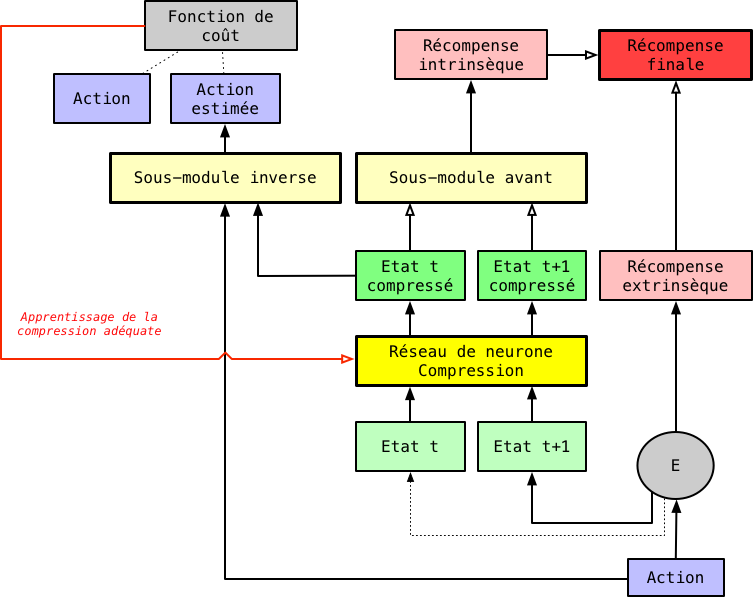
\includegraphics[scale=.4]{./assets/CURIOSITY/curiosity2.png}
        \caption{Schéma finale du module de curiosité mise en place}
    \end{center}
\end{figure}

Le module de curiosité est plus complexe que celui présenté ci-dessus néanmoins le module présenté représente l'idée globale de l'algorithme. Ce module de curiosité a été testé conjointenement avec l'A3C-LSTM-GAE avec les environnements Vizdoom (Doom) et SE-STAR. Les premiers résultats sont encourageants mais il faudra rêgler les quelques problèmes d'interface entre SE-STAR et notre contrôleur pour véritable tester la conjonction des deux algorithmes sont des environnements 3D plus complexe sur SE-STAR. 
